\part{More meshes}
\frame{\partpage}

\begin{frame}{SOH CAH TOA}
	\begin{center}
		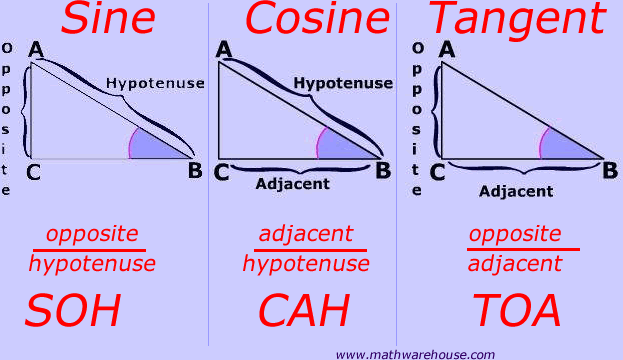
\includegraphics[width=\textwidth]{sohcahtoa}
	\end{center}
\end{frame}

\begin{frame}{Drawing a circle}
	\begin{columns}
		\begin{column}{0.48\textwidth}
			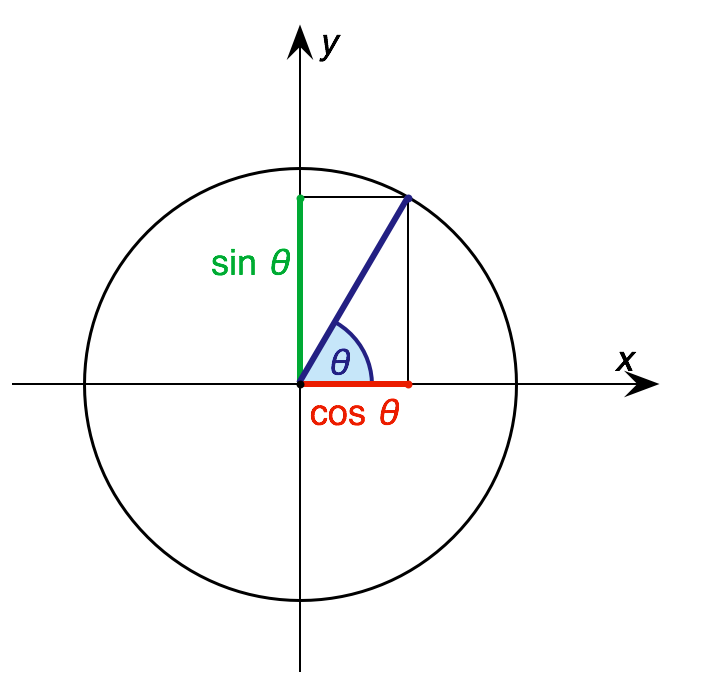
\includegraphics[width=\textwidth]{unit_circle}
		\end{column}
		\begin{column}{0.48\textwidth}
			\pause Circle of \textbf{radius} $r$
			
			\pause $\therefore$ hypotenuse = $r$
			
			\vspace{2ex}
			
			\pause $\cos \theta = \frac{\text{adjacent}}{\text{hypotenuse}} = \frac{x}{r}$
			
			\pause $\therefore x = r \cos \theta$
			
			\vspace{2ex}
			
			\pause $\sin \theta = \frac{\text{opposite}}{\text{hypotenuse}} = \frac{y}{r}$
			
			\pause $\therefore y = r \sin \theta$

			\vspace{2ex}
			
			\pause NB: this works even if $\cos \theta$ and/or $\sin \theta$ are negative
				(i.e.\ if $\theta$ is not between $0^\circ$ and $90^\circ$)
		\end{column}
	\end{columns}
\end{frame}

\begin{frame}{Drawing a cylinder}
	\begin{center}
		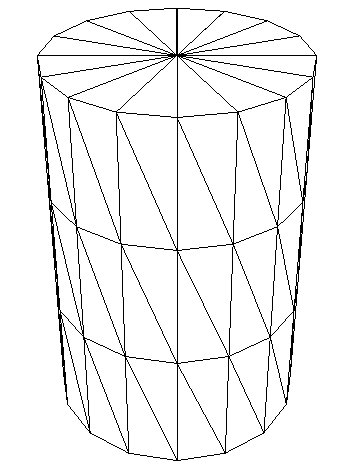
\includegraphics[height=0.8\textheight]{cylinder}
	\end{center}
\end{frame}

\begin{frame}{Drawing a sphere}
	\begin{center}
		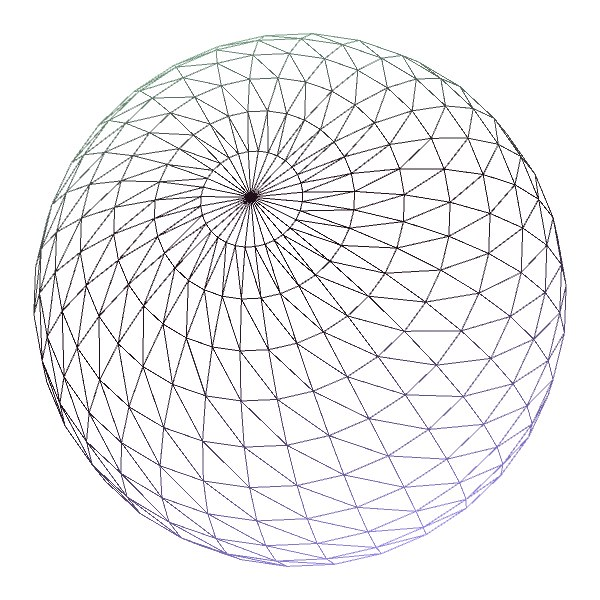
\includegraphics[height=0.8\textheight]{sphere}
	\end{center}
\end{frame}

